\section{Probability}
\begin{outline}

\0
\subsection{Probability reiterated}
	\1 Definitions
		\2 \textbf{Trial: } A trial is a single experiment, such as a single flip of a coin.
		\2 \textbf{Sample space: } The sample space is the list of potential outcomes from an experiment.
		\2 \textbf{Outcome: } An outcome is a possible result of an experiment.
		\2 \textbf{Event: } An event is the list of favourable outcomes.
		\2 \textbf{Equally likely outcomes: } Equally likely outcomes are outcomes that have the same chance of happening.
	\1 Chance
		\2 Chance is a numerical value based on a scale from 0 to 1 that represents probability. 0 represents impossible, while 1 represents certain.
	\1 Calculating theoretical probabilities
		\2 The probability of an event in which outcomes have equal chance is calculated by dividing the number of favourable outcomes by the total number of outcomes.
			\3 Equation
				\[Pr(Event) = \frac{\text{Number of favourable outcomes}}{\text{Total number of outcomes}}\]
	\1 Calculating experimental probabilities
		\2 The probability of experiments only differ to theoretical probability in that experimental probability uses the results of an experiment, rather than relying on results that are purely theoretical with no real application. The calculation of experimental probability differs only slightly from theoretical probability in that instead of dividing the number of favourable outcomes by the total number of outcomes, it uses the total number of trials.
			\3 Equation
				\[Pr(Event) = \frac{\text{Number of favourable outcomes}}{\text{Total number of trials}}\]

\0
\subsection{Unions and intersections}
	\1 Set notation
		\2 \textbf{Set: } A set is a collection or group of elements that can include numbers, letters or other objects.
		\2 \textbf{Sample space: } The sample space, denoted by $\xi$, is the set of all possible elements or objects considered in a particular situation.
		\2 \textbf{Null set: } A null or empty set is a set with no elements and is represented by either $\varnothing$ or $\{\ \ \}$.
		\2 \textbf{Complement: } The complement is everything that isn't the event in question. The complement is represented as an $'$ after the letter, such as $A'$ compared to $A$.
		\2 \textbf{Union: } All elements that belong to either events $A$ or $B$ make up the union. A union is represented as $A\ \cup\ B$.
		\2 \textbf{Intersection: } All elements that belong to both $A$ and $B$ make up the intersection. An intersection is represented as $A\ \cap\ B$.
		\2 \textbf{Mutual exclusion: } Two sets $A$ and $B$ are mutually exclusive if they have no elements in common, meaning $A\ \cap\ B = \varnothing$.
	\1 Venn diagrams
		\2 Venn diagrams are used to illustrate how the elements in the sample space are distributed among the events.
\begin{center}
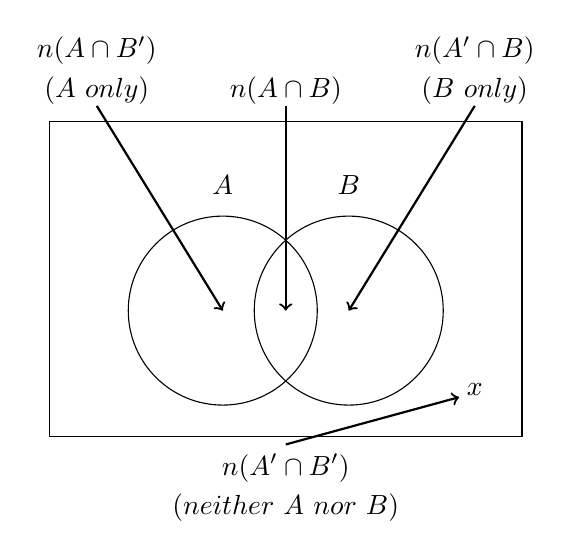
\begin{tikzpicture}[scale=2]
\draw (-1.5,-1) rectangle (1.5,1);
\draw (-0.4,-0.2) circle [radius=0.6];
\draw (0.4,-0.2) circle [radius=0.6];
\node at (-0.4,0.6) {$A$};
\node at (0.4,0.6) {$B$};
\node at (0,1.2) {$n(A \cap B)$};
\node at (-1.2,1.45) {$n(A \cap B')$};
\node at (-1.2,1.2) {$(A\ only)$};
\node at (1.2,1.45) {$n(A' \cap B)$};
\node at (1.2,1.2) {$(B\ only)$};
\node at (1.2, -0.7) {$x$};
\node at (0, -1.2) {$n(A' \cap B')$};
\node at (0, -1.45) {$(neither\ A\ nor\ B)$};
\draw[thick,->] (1.2,1.1) -- (0.4,-0.2);
\draw[thick,->] (-1.2,1.1) -- (-0.4,-0.2);
\draw[thick,->] (0,1.1) -- (0,-0.2);
\draw[thick,->] (0,-1.05) -- (1.10,-0.75);
\end{tikzpicture}
\end{center}
	\1 Listing sets
		\2 Listing sets can be useful in dealing with probability by allowing easier calculation of $Pr(Event)$ probabilities. A good way of dealing with sets is to visualise them as a Venn diagram, however everything involved can be done without visualisation. Firstly, at least in probability involving two events, it is necessary to identify the elements common to both events. With that one can find $A \cup B$, which allows $A' \cap B'$ (the elements outside event $A$ and $B$) to be found.
			\3 Example
\begin{center}
				\[\text{$A$ and $B$ involve numbers taken from integers 1:10}\]
\end{center}
				\[A = \{1,2,3,4,5,6\}\]
				\[B = \{1,3,7,8\}\]
				\[A \cap B = \{1,3\}\]
				\[A \cup B = \{1,2,3,4,5,6,7,8\}\]
				\[A' \cap B' = \{9,10\}\]
	\1 Two-way tables
		\2 Two-way tables are useful tools for organising probability data. They allow for easy mental extrapolation of all probability data when starting with little information.
\begin{center}
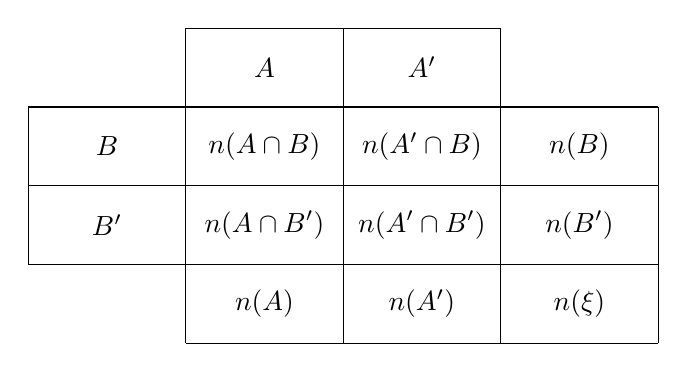
\begin{tikzpicture}[scale=0.5]
\draw (4,0) -- (12,0);
\draw (0,-2) -- (16,-2);
\draw (0,-4) -- (16,-4);
\draw (0,-6) -- (16,-6);
\draw (4,-8) -- (16,-8);
\draw (0,-2) -- (0,-6);
\draw (4,0) -- (4,-8);
\draw (8,0) -- (8,-8);
\draw (12,0) -- (12,-8);
\draw (16,-2) -- (16,-8);
\node at (6,-1) {$A$};
\node at (10,-1) {$A'$};
\node at (2,-3) {$B$};
\node at (6,-3) {$n(A \cap B)$};
\node at (10,-3) {$n(A' \cap B)$};
\node at (14,-3) {$n(B)$};
\node at (6,-5) {$n(A \cap B')$};
\node at (10,-5) {$n(A' \cap B')$};
\node at (14,-5) {$n(B')$};
\node at (2,-5) {$B'$};
\node at (6,-7) {$n(A)$};
\node at (10,-7) {$n(A')$};
\node at (14,-7) {$n(\xi)$};
\end{tikzpicture}
\end{center}	

\0
\subsection{The addition rule}
	\1 The addition rule states that the probability of $A \cap B$ taken away from $A$ added to the probability of $B$ is the same as $A \cup B$. The removal of $A \cap B$ is necessary as $A$ and $B$ both contain $A \cap B$, so subtraction is essential to avoid duplication of $A \cap B$.
	\1 Equation
		\[Pr(A \cup B) = Pr(A) + Pr(B) - Pr(A \cap B)\]
	\1 If A and B are mutually exclusive then:
		\[Pr(A \cap B) = 0\]
		\[Pr(A \cup B) = Pr(A) + Pr(B)\]

\0
\subsection{Conditional probability}
	\1 What is conditional probability
		\2 Conditional probability is probability that an event occurs given that another event has already occurred. The probability of event A occurring given that event B has occurred is denoted by $Pr(A|B)$. $Pr(A|B)$ is read as `the probability of A given B'.
			\3 Equation
				\[Pr(A|B) = \frac{Pr(A \cap B)}{Pr(B)}\ and\ Pr(B|A) = \frac{Pr(A \cap B)}{Pr(A)}\]

\0
\subsection{Multiple events using tables}
	\1 Tables with and without replacement
		\2 Replacement means outcomes can be repeated.
		
\begin{center}
Two selections are made from the digits \{1, 2, 3\}:
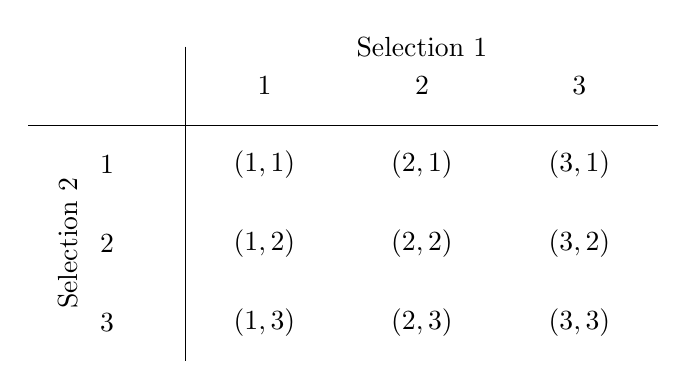
\begin{tikzpicture}[scale=0.5]
\draw (4, 0)--(4,-8);
\draw (0, -2)--(16,-2);
\node at (10,0){Selection $1$};
\node at (1,-5)[rotate=90]{Selection $2$};
\node at (6,-1){$1$};
\node at (10,-1){$2$};
\node at (14,-1){$3$};
\node at (2,-3){$1$};
\node at (2,-5){$2$};
\node at (2,-7){$3$};
\node at (6,-3){$(1,1)$};
\node at (10,-3){$(2,1)$};
\node at (14,-3){$(3,1)$};
\node at (6,-5){$(1,2)$};
\node at (10,-5){$(2,2)$};
\node at (14,-5){$(3,2)$};
\node at (6,-7){$(1,3)$};
\node at (10,-7){$(2,3)$};
\node at (14,-7){$(3,3)$};
\end{tikzpicture}
\end{center}

		\2 No replacement means that outcomes cannot be repeated. Every instance where the same event happens twice, such as $(1,1)$, $(2,2)$, and so on, must be crossed out, or otherwise notated to be an impossibility on the table, as they cannot happen.
		
\begin{center}
Two selections are made from the digits \{1, 2, 3\}:
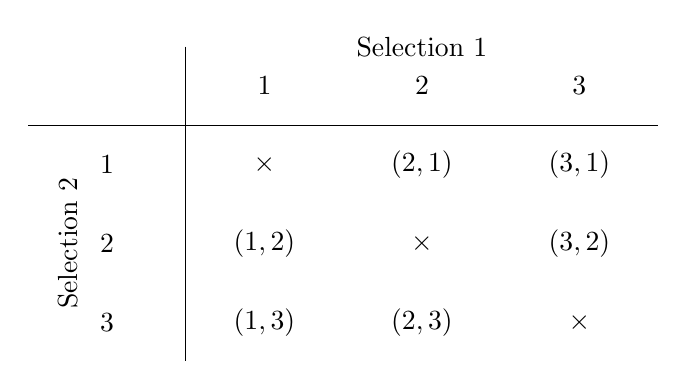
\begin{tikzpicture}[scale=0.5]
\draw (4, 0)--(4,-8);
\draw (0, -2)--(16,-2);
\node at (10,0){Selection $1$};
\node at (1,-5) [rotate=90] {Selection $2$};
\node at (6,-1){$1$};
\node at (10,-1){$2$};
\node at (14,-1){$3$};
\node at (2,-3){$1$};
\node at (2,-5){$2$};
\node at (2,-7){$3$};
\node at (6,-3){$ \times $};
\node at (10,-3){$(2,1)$};
\node at (14,-3){$(3,1)$};
\node at (6,-5){$(1,2)$};
\node at (10,-5){$ \times $};
\node at (14,-5){$(3,2)$};
\node at (6,-7){$(1,3)$};
\node at (10,-7){$(2,3)$};
\node at (14,-7){$ \times $};
\end{tikzpicture}
\end{center}

\0
\subsection{Using tree diagrams}
	\1 Applications
		\2 Tree diagrams can be used to list sample spaces for experiments involving two or more components. Branches can be used to describe the chance of the outcome at each step, and can be used to identify whether an experiment takes into account replacement or no replacement. Probability for the final outcomes may be obtained by multiplying the branch probabilities.
			\3 With replacement

\begin{center}
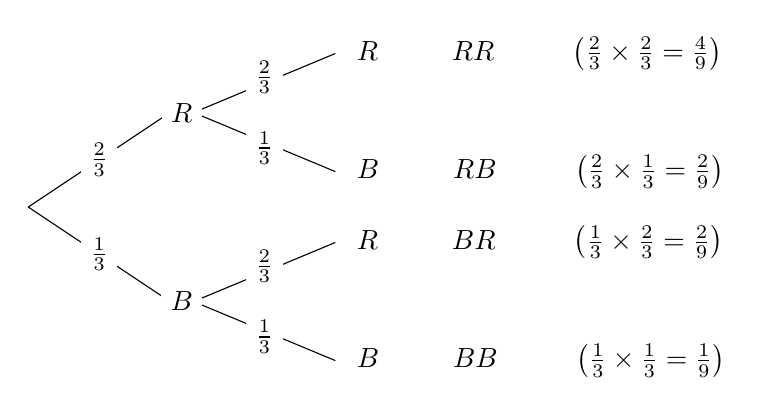
\begin{tikzpicture}[scale=0.3]
\draw (0,0)--(6,4);
\node at (3,2) [fill=white] {$\frac{2}{3}$};
\draw (7,4)--(13,6.5);
\node at (10,5.5) [fill=white] {$\frac{2}{3}$};
\draw (7,4)--(13,1.5);
\node at (10,2.5) [fill=white] {$\frac{1}{3}$};
\draw (0,0)--(6,-4);
\node at (3,-2) [fill=white] {$\frac{1}{3}$};
\draw (7,-4)--(13,-1.5);
\node at (10,-2.5) [fill=white] {$\frac{2}{3}$};
\draw (7,-4)--(13,-6.5);
\node at (10,-5.5) [fill=white] {$\frac{1}{3}$};
\node at (6.5,4) [fill=white] {$R$};
\node at (6.5,-4) [fill=white] {$B$};
\node at (13.5,6.5)[anchor=west]{$R\ \ \ \ \ \ \ \ RR\ \ \ \ \ \ \ \ \left(\frac{2}{3}\times\frac{2}{3} = \frac{4}{9}\right)$};
\node at (13.5,1.5)[anchor=west]{$B\ \ \ \ \ \ \ \ RB\ \ \ \ \ \ \ \ \left(\frac{2}{3}\times\frac{1}{3} = \frac{2}{9}\right)$};
\node at (13.5,-1.5)[anchor=west]{$R\ \ \ \ \ \ \ \ BR\ \ \ \ \ \ \ \ \left(\frac{1}{3}\times\frac{2}{3} = \frac{2}{9}\right)$};
\node at (13.5,-6.5)[anchor=west]{$B\ \ \ \ \ \ \ \ BB\ \ \ \ \ \ \ \ \left(\frac{1}{3}\times\frac{1}{3} = \frac{1}{9}\right)$};
\end{tikzpicture}
\end{center}
			\3 Without replacement
\begin{center}
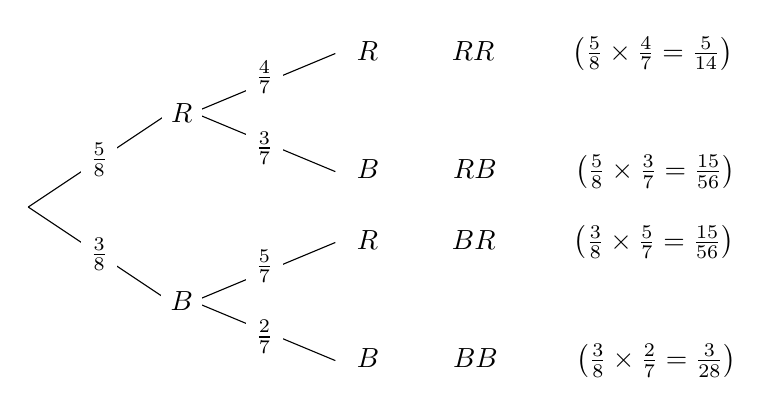
\begin{tikzpicture}[scale=0.3]
\draw (0,0)--(6,4);
\node at (3,2) [fill=white] {$\frac{5}{8}$};
\draw (7,4)--(13,6.5);
\node at (10,5.5) [fill=white] {$\frac{4}{7}$};
\draw (7,4)--(13,1.5);
\node at (10,2.5) [fill=white] {$\frac{3}{7}$};
\draw (0,0)--(6,-4);
\node at (3,-2) [fill=white] {$\frac{3}{8}$};
\draw (7,-4)--(13,-1.5);
\node at (10,-2.5) [fill=white] {$\frac{5}{7}$};
\draw (7,-4)--(13,-6.5);
\node at (10,-5.5) [fill=white] {$\frac{2}{7}$};
\node at (6.5,4) [fill=white] {$R$};
\node at (6.5,-4) [fill=white] {$B$};
\node at (13.5,6.5)[anchor=west]{$R\ \ \ \ \ \ \ \ RR\ \ \ \ \ \ \ \ \left(\frac{5}{8}\times\frac{4}{7} = \frac{5}{14}\right)$};
\node at (13.5,1.5)[anchor=west]{$B\ \ \ \ \ \ \ \ RB\ \ \ \ \ \ \ \ \left(\frac{5}{8}\times\frac{3}{7} = \frac{15}{56}\right)$};
\node at (13.5,-1.5)[anchor=west]{$R\ \ \ \ \ \ \ \ BR\ \ \ \ \ \ \ \ \left(\frac{3}{8}\times\frac{5}{7} = \frac{15}{56}\right)$};
\node at (13.5,-6.5)[anchor=west]{$B\ \ \ \ \ \ \ \ BB\ \ \ \ \ \ \ \ \left(\frac{3}{8}\times\frac{2}{7} = \frac{3}{28}\right)$};
\end{tikzpicture}
\end{center}

\0
\subsection{Independent events}
	\1 Definition
		\2 Two events are independent if the outcome of one event does not change the probability of obtaining the other event. There are two equations to check the independency of $A$ regarding $B$ or $B$ regarding $A$
			\3 Equation
				\[Pr(A | B) = Pr(A) \text{\ \ \ \ OR\ \ \ \ } Pr(B | A) = Pr(B)\]
				\[Pr(A \cap B) = Pr(A) \times Pr(B)\]
		\2 For multiple events with selection made with replacement, events are independent. For multiple events with selection made without replacement, events are not independent.

\end{outline}
